% Template for ISBI paper; to be used with:
%          spconf.sty  - ICASSP/ICIP LaTeX style file, and
%          IEEEbib.bst - IEEE bibliography style file.
% --------------------------------------------------------------------------
\documentclass{article}
\usepackage{spconf,amsmath,graphicx,hyperref}

% Example definitions.
% --------------------
\def\x{{\mathbf x}}
\def\L{{\cal L}}

% Title.
% ------
\title{Inexact Graph Matching for Neuron Tracking in Calcium Imaging}
%
% Single address.
% ---------------
\name{K. V. Busum$^1$, W. D. Tracy$^2$, L. He$^2$, S. Gulyanon$^3$, and G. Tsechpenakis$^1$ \thanks{This work is supported by NSF/DBI [$\#$1252597]: `CAREER: Modeling the structure and dynamics of neuronal circuits in the \emph{Drosophila} larvae using image analytics' awarded to G. Tsechpenakis.} \vspace{-5pt}}
\address{\small{$^1$Computer and Information Science Department, Indiana University-Purdue University Indianapolis, USA;} \\
	\small{$^2$ Department of Biology, Indiana University, USA;} \\
	\small{$^3$Data Science and Innovation Program, Faculty of Science and Technology, Thammasat University, Thailand;} \vspace{-2pt} \\}
%
% For example:
% ------------
%\address{School\\
%	Department\\
%	Address}
%
% Two addresses (uncomment and modify for two-address case).
% ----------------------------------------------------------
%\twoauthors
%  {A. Author-one, B. Author-two\sthanks{Thanks to XYZ agency for funding.}}
%	{School A-B\\
%	Department A-B\\
%	Address A-B}
%  {C. Author-three, D. Author-four\sthanks{The fourth author performed the work
%	while at ...}}
%	{School C-D\\
%	Department C-D\\
%	Address C-D}
%
% More than two addresses
% -----------------------
% \name{Author Name$^{\star \dagger}$ \qquad Author Name$^{\star}$ \qquad Author Name$^{\dagger}$}
%
% \address{$^{\star}$ Affiliation Number One \\
%     $^{\dagger}$}Affiliation Number Two
%
\begin{document}
%\ninept
%
\maketitle
%
\begin{abstract}	
Calcium imagery captures both the structure and functionality of neurons. Tracking neurons on such images gives us a glimpse of how the locomotion in Drosophila larvae is executed and gain insights into the relationship between the two aspects of neurons. This problem is challenging due to (a) only active neurons are visible in calcium images, and (b) severe deformation from peristaltic locomotion. We propose the novel neuron tracking method based on the inexact graph matching over a set of graphs, each representing the neuron at one timestep. Computed using A*-beamsearch, the optimal match minimizes the graph edit distance. It incorporates the tissue deformation, local image feature, neuronal morphology, and local characteristics of neurons. Unlike existing methods, ours has no hard shape constraints so it requires no meticulous conditions for each type of neurons. Our results show the performance of our method and compare it with existing frameworks using sample calcium volumes of larval Drosophila sensory neurons.

\end{abstract}
%
\begin{keywords}
neuron tracking, calcium images, inexact graph matching, graph edit distance, A*-beamsearch
\end{keywords}
%
\section{Introduction}
\label{sec:intro}

High speed confocal imaging of calcium dynamics in proprioceptive neurons of larval Drosophila allows us to observe both the morphology and neuronal activity simultaneously. These sensory neurons lie directly beneath the cuticle and epidermis, which are optically transparent, so they are observable \emph{in vivo}. The responses of calcium images are proportional to neuronal activities on neurites. By measuring displacements of proprioceptive sensory dendrites and changes in activity levels over neurites, we are able to relate the direction of locomotion to these two properties and gain insights into the underlying molecular mechanisms that determine the responses of the proprioceptive cells \cite{He2019}.

Neuron tracking \emph{in vivo} is a challenging problem by itself due to the crawling locomotion of Drosophila larvae. It produces a movement pattern that alternates between stationary poses and severe deformations. Second issue is related to the unique characteristic of calcium images, where low levels of neuron activation yield low intensity. This gives difficulty in distinguishing between the neuron volume and background because of low contrast. It also introduces changes in intensity during the locomotion and inhomogeneous responses over dendrites from cellular mechanism. Other issues are noisy calcium image sequences and low resolution along the Z-axis owing to imaging system limitations.

Conventional tracking approaches, i.e., tracking-by-detection \cite{Gulyanon2016, Glowacki2018} and optical flow-based \cite{Chen2016} methods, fail to detect and track neurites under spatially inhomogeneous intensity ambiguities of calcium images and wave-like movement patterns of Drosophila larvae because these methods assume temporal intensity smoothness constraint \cite{Gulyanon2018a}. Previous approaches address these problems by enforcing hard shape constraints, e.g., the proximity between dendrites, to avoid invalid tracking results through techniques like deformable models. For example, the method in \cite{Gulyanon2018a} tracks parts of the articulated body that represents the neurite centerlines, while authors in \cite{Gulyanon2019} use the accordion model, a variant of an articulated surface, to capture the tissue deformation of the surface to which the neurons are attached. The hard constraints for topology produce robust tracking results that are visually pleasing at the cost of poor accuracy under abrupt deformations. 

In this paper, we tackle the neuron tracking problem over calcium images as the \emph{inexact graph matching} (IGM) problem, where the segmentation of neuron in each timestep is represented by a graph. IGM finds the mapping of nodes between two graphs of the same neuron at consecutive timesteps by optimizing a certain affinity criterion, the customized \emph{graph edit distance} (GED). It takes into account the tissue deformation, local image feature, neuronal morphology, and local characteristics of neurons. This formulation utilizes the soft shape constraints embedded in the GED instead of the hard shape constraints so the rigorous topology conditions are no longer needed. Techniques for GED computation are reviewed in \cite{Yan2016, Gao2010} and A*-beamsearch is suitable for our task since it is the simple but effective optimization algorithm that can accommodate many-to-many relationship \cite{Morrison2015, Neuhaus2006}.

\begin{figure}[t!]
	\centering
	\vspace{-10pt}
	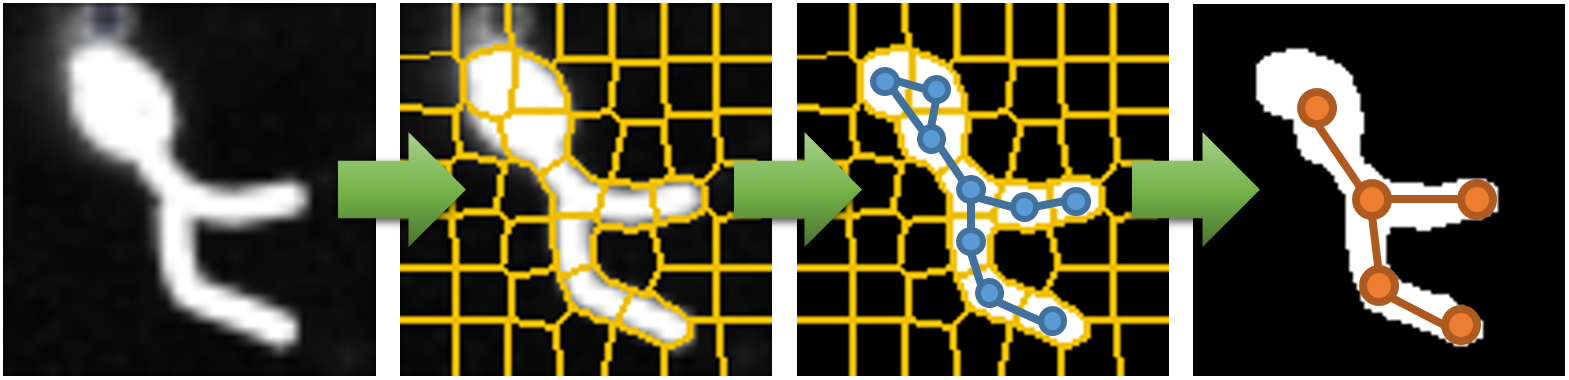
\includegraphics[width=\columnwidth]{img/method.png}
	\vspace{-20pt}
	\caption{\small{From left to right. Input image, the ``frame'' graph, the ``template'' graph, and the aligned neuron trace. Yellow lines show the boundary of superpixels. Blue color shows the ``frame'' graph and ``template'' subgraph. Orange color shows the trace result.}}
	\label{fig:method}
	\vspace{-10pt}
\end{figure}


\section{Method}
Let $\mathcal{I} = \{ \mathcal{I}^{(t)} \}$ denote the calcium image stack sequence, where $t = 0,1,\dots,T$. To make the problem feasible, we require the initial morphology of the neuron, $\mathcal{G} = \{ V_\mathcal{G}, E_\mathcal{G} \}$. A \emph{graph} is denoted by $G = \{V, E\}$, where $V$ is the set of nodes and $E \subset V \times V$ is the set of edges of graph $G$. Every frame is represented by the ``frame'' graph, where nodes are the non-overlapping regions in the image. The segmentation of the neuron is represented by the ``template'' graph, the subgraph of ``frame'' graph depicting the neuron.

Let $G'_{t-1}$ and $G'_t$ are the ``template'' graphs of the same neuron at consecutive timesteps. We formulate the tracking problem as finding $G'_t$ and a sequence of graph edit operations, $P$, that transforms $G'_{t-1}$ into $G'_t$, with the minimum GED, $\delta(G'_{t-1}, G'_t)$:
\begin{equation} \label{eq:ged}
\delta(G'_{t-1}, G'_t) = \min_P \sum_{(u \rightarrow v) \in P} c(u \rightarrow v)
\end{equation}
where nodes $u \in V'_{t-1}$ and $v \in V'_t$ are a correspondence; and $c(u \rightarrow v)$ is the cost of the graph edit operation that maps node $u$ to $v$, which depends on the affinity between $u$ and $v$ described in Sec.~\ref{sec:cost}. Finally, we recover the trace in every frame by aligning dendrites of the initial morphology, $\mathcal{G}$, to the binary image of neuron (fig.~\ref{fig:method}).



\subsection{Creating ``Frame'' Graph}
%First, we convert every frame into the graph representation, $G_t = \{ V_t, E_t \}$. 
The ``frame'' graph, $G_t = \{ V_t, E_t \}$, of the image stack at time $t$ is computed by the superpixel segmentation \cite{Li2015, Chen2017}. Due to the imaging system limitation, the maximum intensity projection of calcium image stack, $I_t = f(\mathcal{I}^{(t)})$, is used instead of the raw input volume. The set of nodes, $V_t$, is the superpixels over $I_t$, while the set of edges, $E_t$, are computed using Delaunay triangulation over the centroids of superpixels in $V_t$.

\subsection{Initial ``Template'' Graph}
A trace describes the neuron morphology at the structural level, while an image stack describes the neuron at the appearance level. We propose the ``template'' graph that bridges between two levels of representations.

The ``template'' graph at time $t=0$, $G'_0 =  \{V'_0, E'_0 \}$, is the subgraph of $G_0$ corresponded to the initial morphology $\mathcal{G}$. $V'_0 = \{\,v \mid v \text{ overlaps } \mathcal{G}, v \in V_0 \,\}$ is the set of node depicting the initial morphology $\mathcal{G}$. $E'_0$ is the set of edges between adjacent nodes in $V'_0$, $E'_0 = \{\, (u, v) \mid (u, v) \in E_0 ;\; u, v \in V'_0 \,\}$.


\subsection{Tree Search Algorithm} \label{sec:treealgo}
A tree (state space) search algorithm \cite{Morrison2015} is used to find the GED because it is simple, allows the many-to-many mapping function, and makes no assumptions about the problem. Tracking is done by computing the GED between the previous ``template'' graph and the current ``frame'' graph, $\delta (G'_{t-1}, G_t)$. Since the IGM is error tolerant, nodes of the graph do not need to have a correspondence in another graph and the match do not need to be exactly the same. Hence, this computes both $G'_t$ and $P$ simultaneously as $G'_t$ is the subgraph of $G_t$ that has the correspondence in $G'_{t-1}$ with respect to $P$ and $P$ describes the steps to transform from $G'_{t-1}$ to both $G_t$ and $G'_t$. 

The state space consists of a number of possible mappings with different cost (fig.~\ref{fig:treesearch}). The algorithm terminates when every node in $G'_{t-1}$ has at least one correspondence in $G_t$.

%%TODO: add figure describing tree search algorithm
%\begin{figure}[b!]
%	\centering
%	\vspace{-10pt}
%	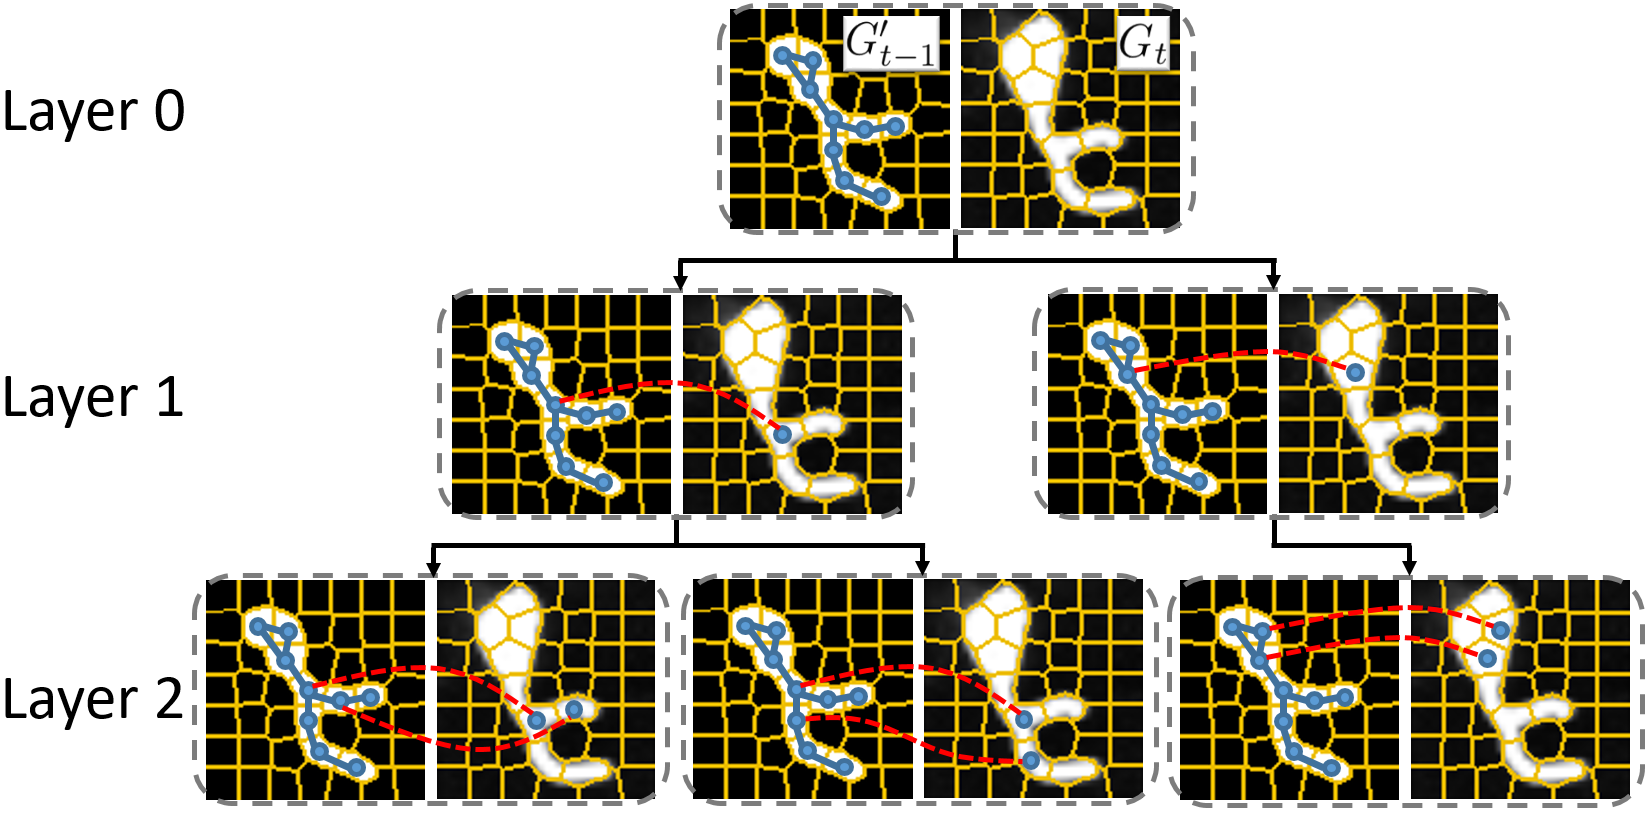
\includegraphics[width=\columnwidth]{img/treesearch.png}
%	\vspace{-20pt}
%	\caption{\small{Tree state space search using A*-beamsearch. The root of the state space represents the mapping with no correspondences. The first layer of states represents mappings with one correspondence, and so on. Red lines show pairs of nodes that are a correspondence. In A*-beamsearch, only a $b$ number of states with the lowest heuristic costs in each layer are explored.}}
%	\label{fig:treesearch}
%	\vspace{-10pt}
%\end{figure}

\begin{figure*}[t!]
	\centering
	\vspace{-10pt}
	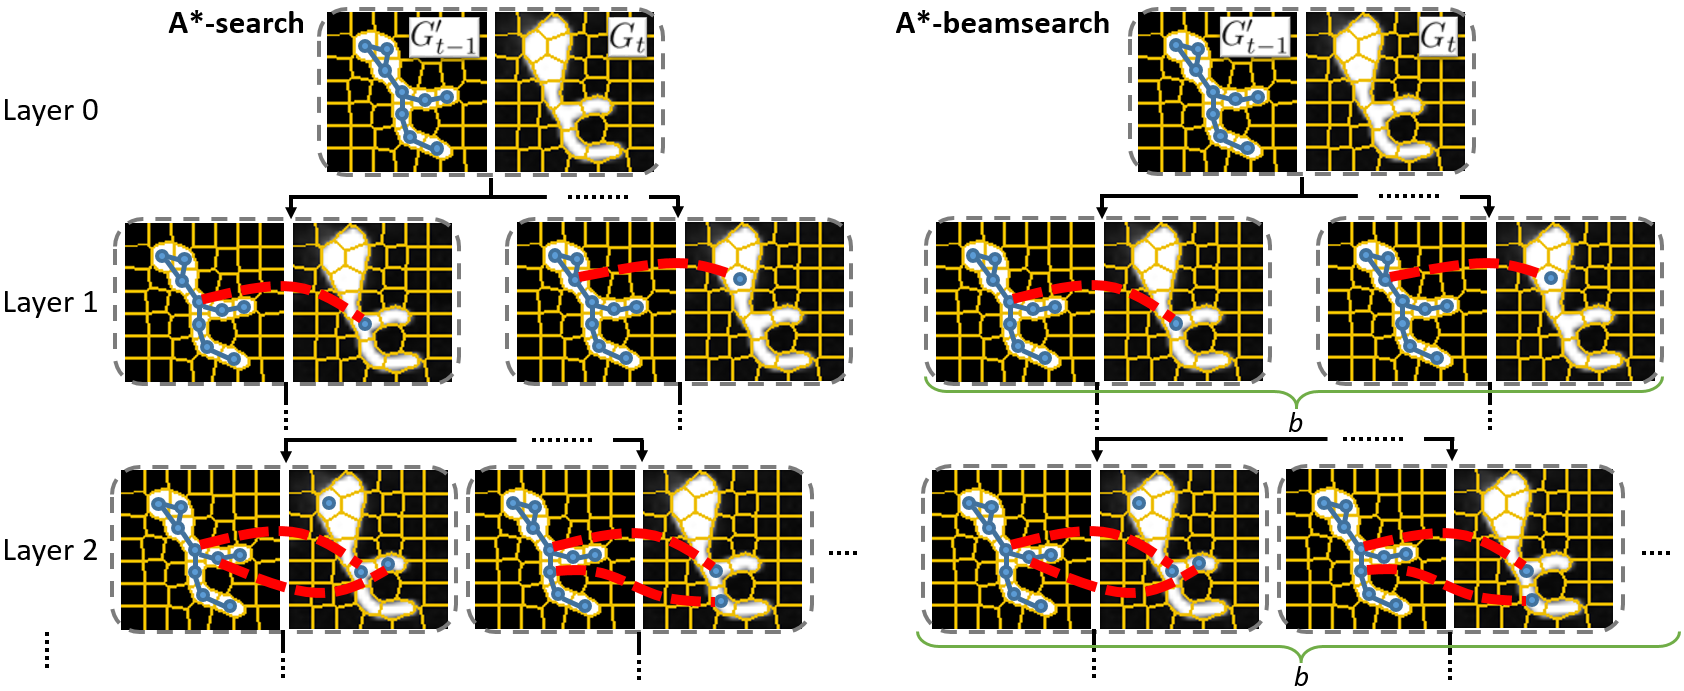
\includegraphics[width=\textwidth]{img/asearch.png}
	\vspace{-20pt}
	\caption{\small{Tree state space search using A*-search (left) and A*-beamsearch (right). The root of the state space represents the mapping with no correspondences. The first layer of states represents mappings with one correspondence, and so on. Red lines show pairs of nodes that are a correspondence. In A*-beamsearch, only a $b$ number of states with the lowest heuristic costs in each layer are explored.}}
	\label{fig:treesearch}
	\vspace{-10pt}
\end{figure*}


A state is produced by adding a new correspondence to the parent state. Let $\psi$ be a function that determines, for a given state/mapping $p$, a set of possible new correspondences that can be added to form new child states. 
\small
\begin{equation}
\psi(p) = \{ \check{V}_{p,t-1} \times \check{V}_{p,t} \} \cup \{ \check{V}_{p,t-1} \times V_{p,t} \} \cup \{ V_{p,t-1} \times \check{V}_{p,t} \}
\end{equation}
\normalsize
where $\check{V}_{p,t}$ is the set of nodes that are not currently mapped and are adjacent to the set of mapped nodes $V_{p,t}$, $\check{V}_{p,t} = \{\, v \mid (u,v) \in E_t, u \in V_{p,t}, v \notin V_{p,t} \,\}$.



\subsection{Fine Tracking: Aligning Dendrites}
%We align dendrites using \cite{Farhand2016}

Consider a set of nodes, $V_d \subset V_\mathcal{G}$, that constitutes a dendrite $d$ in the neuron trace. The nodes corresponding to the dendrite $d$ in the ``template'' graph at time $t = 0$ is $V'_{d,0} = \{\,v \mid v \text{ overlap with } V_d, v \in V_0 \,\}$. For time $t$, $V'_{d,t} = P( V'_{d,t-1})$. The alignment between dendrite at consecutive timesteps is done by registering patches from $V'_{d,t-1}$ to $V'_{d,t}$ using techniques like free-form deformation (FFD) \cite{Rueckert1999}.


\section{Optimization} 
A tree search algorithm in Sec.~\ref{sec:treealgo} must be efficient to make this method feasible since there are $|V'_{t-1}||V_t|$ possible correspondences. Fortunately, many states/mappings have no meaningful interpretation, e.g., mappings that produce unconnected dendrites, and neurons usually occupy small regions in the image stacks. Hence, there are a limited number of candidate mappings to need to be explored. 

In this work, the computation of GED uses the A*-beamsearch algorithm \cite{Neuhaus2006} with node grouping, that only explores the most likely and meaningful states and allows many-to-many mapping solution.

\subsection{A* Search}
The A* or the best-first search algorithm \cite{hart1968} finds an optimal path from a state space based on a heuristic function, which estimates the expected costs of the best route from the root through the current state (partial solution) to a leaf state (complete solution). At each step during tree state space traversal, the most promising state --- the lowest heuristic cost --- from the set of child states is chosen. Hence, at any state $p$, A* algorithm selects the path that minimizes the following cost:
\begin{equation} \label{eq:a*}
f(p) = g(p) + h(p)
\end{equation}
where $g(p)$ is the cost of the optimal path from the root to the current state $p$ and $h(p)$ is the estimated cost from state $p$ to a leaf state. Here, $h(p)$ is defined by the average cost of $g(p)$ times the number of remaining unmapped nodes.

\subsection{Beam Search}
A* search may end up expanding all successor nodes in the search space. In beam search, only a fixed number, $b$ called \emph{beam width}, of states in each layer are explored. We pick the $b$ states with the lowest costs from eq.~\ref{eq:a*} (fig.~\ref{fig:treesearch}), so only states with the most promising partial mappings are explored. Hence, the cost function must reflects the graph similarity, the more similar the graphs are the lower the cost is \cite{Neuhaus2006}.



\section{Cost Function} \label{sec:cost}
The cost function, $c(u \rightarrow v)$, of the state $p$ takes a correspondence and returns a single value measuring the compatibility between node $u$ and $v$ based on the tissue deformation, local image feature, neuronal morphology, and local characteristics of neurons. Edge comparison is not meaningful here since edge captures the relationship between nodes but the correspondent nodes are not guaranteed to be the same. However, we still need the neighborhood information that edges have. Thus, we aggregate the edge information and embed them in the node descriptor. 

The match is inexact so a node may have multiple correspondences. Thus, we must define the cost function between two nodes (one-to-one function) and between a node and a group of nodes (many-to-one/one-to-many functions).

\subsection{Node to Node}
The first part of the node descriptor is the image feature considered through intensity and local orientation. The \textbf{average intensity} of node $v_i \in V_t$ is defined by,
\begin{equation}
I_t(v_i) = \frac{1}{|S(v_i)|}\sum_{x \in S(v_i)} I_t(x)
\end{equation} 
where $S(v_i)$ is the set of pixels in the superpixel corresponded to node $v_i$. The \textbf{average eigenvector} of node $v_i \in V_t$ indicates the local neurite orientation via eigenvalue analysis of the Hessian matrix \cite{frangi1998},
\begin{equation}
F(v_i) = \frac{1}{|S(v_i)|}\sum_{x \in S(v_i)} \hat{\textbf{u}}_{x,1}
\end{equation}
where $\hat{\textbf{u}}_{x,1}$ is the eigenvector with the smallest eigenvalue at pixel $x$.
%where let $\lambda_{s,x,k}$ denote the eigenvalue corresponding to the $k$-th normalized eigenvector $\hat{\textbf{u}}_{s,x,k}$
%of the Hessian matrix of the image $\mathcal{H}_{x,k}$ all computed at scale $s$ on pixel $x$. 
%\begin{equation}
%\lambda_{x,k} = \max_{s_{min} \le s \le s_{max}} \lambda_{s,x,k}
%\end{equation}
%$\lambda_{x,k}$ is the eigenvalue with the $k$-th smallest magnitude and $\hat{\textbf{u}}_{x,k}$ are their corresponding eigenvectors.
To include the local characteristics, the \textbf{relation to neighbors} measures the intensity similarity between a node and its neighborhood. To compute, first find the location $L_{ij}$ and magnitude $M_{ij}$ based on the average intensity similarity for each neighbor $v_j$ of $v_i$, $(v_i, v_j) \in E_t$,
\begin{equation}
\begin{aligned}
L_{ij} & = C(v_j) - C(v_i) \\
M_{ij} & = 1 - \| I_t(v_j) - I_t(v_i) \|
\end{aligned}
\end{equation}
where $C(v_i)$ is the centroid of the superpixel corresponded to node $v_i$ denoted by the $xy$-coordinate, $(x_i, y_i)$.

Then, a histogram is created to encode the relation to neighboring superpixels, similar to the orientation histogram in SIFT \cite{Lowe1999}. In this histogram, the 360 degrees of $L_{ij}$ direction are broken into 8 bins (each 45 degrees). The amount added to the bin depends on the magnitude projected in the bin's direction.

To achieve rotation independence, make the orientation relative to the keypoint's orientation by subtracting the keypoint's rotation from each orientation. The keypoint is the bin with the highest magnitude.

To achieve illumination dependence, threshold the magnitudes that are too big.

Similarly, \textbf{relation to mapping} indicates the proximity between $v_i$ and mapped nodes. This helps distinguish nodes along ambiguous regions like dendrites since points along the dendritic line segment have similar properties. It is a histogram of mapped neighbors' orientation weighted by the inverse of distance $H_{ij}$, where $v_j \in V_{p,t}$.
\begin{equation}
H_{ij} = \frac{1}{ \| L_{ij} \| }
\end{equation}

\textbf{Smooth deformation} keeps the change in deformation low over space. For $u_i^{t-1} \in \check{V}_{p,t-1}$ and $v_i^t \in \check{V}_{p,t}$, the deformation of the correspondence $i$ is defined as,
\begin{equation}
d_i = C(u_i^{t-1}) - C(v_i^t)
\end{equation}

For $(u_i^{t-1}, u_j^{t-1}) \in E'_{t-1}$ and $(v_i^t, v_j^t) \in E_t$, where $u_i^{t-1}$ and $v_i^t$ are correspondence we are considering; $u_j^{t-1} \in V_{p,t-1}$ and $v_j^t \in  V_{p,t}$ are the adjacent correspondences we found earlier. Then, the change in deformation at correspondence $i$ is:
\begin{equation}
D_i = \sum_{d_j} \| d_j - d_i \|
\end{equation}

Hence, the node descriptor $\alpha(v_i)$ is defined as the tuple of 19 numbers: average intensity $I_t(v_i)$, the orientation of the average eigenvector $F(v_i)$ in radian, smooth deformation $T_i$, and the values in both histograms' bins.

The cost of substituting node $(u,v) \in \{ \check{V}_{p,t-1} \times \check{V}_{p,t} \}$ is defined based on cosine similarity as follows:
\begin{equation}
c(u \rightarrow v) = 1 - \frac{\sum_{i=1}^N \alpha_i(u)\alpha_i(v)}{\sqrt{\sum_{i=1}^N \alpha_i^2(u)}\sqrt{\sum_{i=1}^N \alpha_i^2(v)}}
\end{equation}

%TODO add figure showing cost function

\subsection{Node to Group of Nodes}
The node grouping is needed for finding many-to-many relationship between frames in an efficient way, similar to \cite{Morrison2015}.

The cost of substituting node $(u,v) \in \{ \check{V}_{p,t-1} \times V_{p,t} \}$ is defined based on cosine similarity as before but the descriptor of $u$ must take into account other correspondences of $v$.

Let $\hat{u}$ is the set of nodes correspondence to $v$, $\hat{u} = \{\, w \mid (w \rightarrow v) \in p \,\} \cup \{u\}$. Then, $\alpha(\hat{u})$ denotes the group-of-node descriptor. \textbf{Average intensity} and \textbf{average eigenvector} of a group of nodes are defined as,
\begin{equation}
\begin{aligned}
I_t(\hat{u}) & = \frac{1}{|S(\hat{u})|}\sum_{x \in S(\hat{u})} I_t(x) \\
F(\hat{u}) & = \frac{1}{|S(\hat{u})|}\sum_{x \in S(\hat{u})} \hat{\textbf{u}}_{x,1}
\end{aligned}
\end{equation} 

The \textbf{relation to neighbors}, \textbf{relation to mapping}, and \textbf{smooth deformation} are quantified from the neighbors of the group of nodes, ignoring the internal edges within the group; while the centroid is defined as the middle point of the group.

The cost of substituting node $(u,v) \in \{ V_{p,t-1} \times \check{V}_{p,t} \}$ follows the same suit.

%TODO add figure showing correspondence between node and a group of nodes
%TODO clarify correspondence between node and a group of nodes

\section{Results}
%TODO Add result
We validated our method using time-lapse calcium volumes of larval Drosophila dda-E and dda-D sensory neurons. Larvae expressing the genetically encoded calcium sensor GCaMP6.0F in the proprioceptors were observed in 4-D confocal microscopy imagery \cite{He2019}.

\section{Conclusion}
%TODO Add conclusion

% To start a new column (but not a new page) and help balance the last-page
% column length use \vfill\pagebreak.
% -------------------------------------------------------------------------
\vfill
\pagebreak


% References should be produced using the bibtex program from suitable
% BiBTeX files (here: strings, refs, manuals). The IEEEbib.bst bibliography
% style file from IEEE produces unsorted bibliography list.
% -------------------------------------------------------------------------
\bibliographystyle{IEEEbib}
\small{
%TODO recheck reference
%\bibliography{all}
\begin{thebibliography}{10}
	
	\bibitem{He2019}
	L.~He, S.~Gulyanon, M.M. Skanata, D.~Karagyozov, E.S. Heckscher, M.~Krieg,
	G.~Tsechpenakis, M.~Gershow, and W.D. Tracey,
	\newblock ``Direction selectivity in drosophila proprioceptors requires the
	mechanosensory channel {Tmc},''
	\newblock {\em Current Biology}, 29(6):945--956.e3, 2019.
	
%	\bibitem{Gulyanon2015}
%	S.~Gulyanon, N.~Sharifai, S.~Bleykhman, E.~Kelly, M.~D. Kim, A.~Chiba, and G.~Tsechpenakis,
%	\newblock ``Three-dimensional neurite tracing under globally varying contrast,''
%	\newblock {\em in proc. ISBI}, pp. 875--879, 2015.
	
	\bibitem{Gulyanon2016}
	S.~Gulyanon, N.~Sharifai, M.~D. Kim, A.~Chiba, and G.~Tsechpenakis,
	\newblock ``{CRF} formulation of active contour population for efficient three-dimensional neurite tracing,''
	\newblock {\em in proc.  ISBI}, pp. 593--597, 2016.
	
	\bibitem{Glowacki2018}
	P.~{Głowacki}, M.~A. {Pinheiro}, A.~{Mosinska}, E.~{Türetken}, D.~{Lebrecht},
	R.~{Sznitman}, A.~{Holtmaat}, J.~{Kybic}, and P.~{Fua},
	\newblock ``Reconstructing evolving tree structures in time lapse sequences by
	enforcing time-consistency,''
	\newblock {\em TPAMI}, 40(3):755--761, 2018.
	
	\bibitem{Chen2016}
	Q.~Chen and V.~Koltun,
	\newblock ``Full flow: Optical flow estimation by global optimization over
	regular grids,''
	\newblock {\em in proc.  CVPR}, pp. 4706--4714, 2016.
	
%	\bibitem{Bailer2017}
%	C.~Bailer, K.~Varanasi, and D.~Stricker,
%	\newblock ``{CNN}-based patch matching for optical flow with thresholded hinge loss,''
%	\newblock {\em in proc. CVPR}, pp. 2710--2719, 2017.
	
	\bibitem{Gulyanon2018a}
	S.~Gulyanon, L.~He, W.D. Tracey, and G.~Tsechpenakis,
	\newblock ``Neurite tracking in time-lapse calcium images using {MRF}-modeled
	pictorial structures,''
	\newblock {\em in proc. ISBI}, pp. 1564--1568, 2018.
	
	\bibitem{Gulyanon2019}
	S.~Gulyanon, L.~He, W.D. Tracey, and G.~Tsechpenakis,
	\newblock ``Neuron tracking in calcium image stacks using accordion
	articulations,''
	\newblock {\em in proc. ISBI}, 2019.
	
	\bibitem{Yan2016}
	J.~Yan, X.-C. Yin, W.~Lin, C.~Deng, H.~Zha, and X.~Yang,
	\newblock ``A short survey of recent advances in graph matching,''
	\newblock {\em in proc. ICMR}, pp. 167--174, 2016.
	
	\bibitem{Gao2010}
	X.~Gao, B.~Xiao, D.~Tao, and X.~Li,
	\newblock ``A survey of graph edit distance,''
	\newblock {\em Pattern Anal Appl}, 13(1):113--129, 2010.
	
	\bibitem{Morrison2015}
	P.~Morrison and J.J. Zou,
	\newblock ``Inexact graph matching using a hierarchy of matching processes,''
	\newblock {\em Computational Visual Media}, 1(4):291--307, 2015.
	
	\bibitem{Neuhaus2006}
	M.~Neuhaus, K.~Riesen, and H.~Bunke,
	\newblock ``Fast suboptimal algorithms for the computation of graph edit
	distance,''
	\newblock {\em S+SSPR}, pp. 163--172, 2006.
	
	\bibitem{Li2015}
	Z.~Li and J.~Chen,
	\newblock ``Superpixel segmentation using linear spectral clustering,''
	\newblock {\em in proc. CVPR}, pp. 1356--1363, 2015.
	
	\bibitem{Chen2017}
	J.~Chen, Z.~Li, and B.~Huang,
	\newblock ``Linear spectral clustering superpixel,''
	\newblock {\em IEEE Trans Image Process}, 26(7):3317--3330, 2017.
	
	\bibitem{Farhand2016}
	S.~Farhand, S.~Gulyanon, N.~Sharifai, M.~D. Kim, A.~Chiba, and G.~Tsechpenakis,
	\newblock ``Temporal neurite registration using hierarchical alignments,''
	\newblock {\em in proc. ISBI}, pp. 334--338, 2016.
	
%	\bibitem{Rueckert1999}
%	D.~Rueckert, L.I. Sonoda, C.~Hayes, D.L.G. Hill, M.O. Leach, and D.J. Hawkes,
%	\newblock ``Nonrigid registration using free-form deformations: Application to
%	breast {MR} images,''
%	\newblock {\em IEEE Trans Med Imag}, 18(8):712--721, 1999.
	
	\bibitem{hart1968}
	P.E. Hart, N.J. Nilsson, and B.~Raphael,
	\newblock ``A formal basis for the heuristic determination of minimum cost
	paths,''
	\newblock {\em IEEE Trans Syst Sci Cybern}, 4(2):100--107, 1968.
	
	\bibitem{frangi1998}
	A.F. Frangi, W.J. Niessen, K.L. Vincken, and M.A. Viergever,
	\newblock ``Multiscale vessel enhancement filtering,''
	\newblock {\em in proc. MICCAI}, pp. 130--137, 1998.
	
	\bibitem{Lowe1999}
	D.G. Lowe,
	\newblock ``Object recognition from local scale-invariant features,''
	\newblock {\em in proc. ICCV}, vol. 2, pp. 1150--1157, 1999.
	
\end{thebibliography}

}

\end{document}
